\documentclass[oneside,11pt]{amsart}
\usepackage[utf8]{inputenc}%
\usepackage[english]{babel}%
\usepackage{amsmath,amssymb,amsthm,amsfonts}%
\usepackage[unicode]{hyperref}%
\usepackage{mathrsfs,bbm}%
\usepackage{paralist}
\usepackage{color}
\usepackage{longtable}
\usepackage{array}
\usepackage{stmaryrd}%
%\usepackage{refcheck}
\usepackage{graphicx}
\usepackage[DIV15]{typearea}
\usepackage{multicol,tikz}
\usepackage{datetime}
\usepackage{cleveref}

\usepackage[shadow]{todonotes}

\usepackage{etoolbox}
\patchcmd{\section}{\scshape}{\large\itshape\bfseries}{}{}

\usepackage{caption}
\captionsetup{labelformat=empty,labelsep=none}

\hypersetup{
  colorlinks=true,
  linkcolor=blue!50!red,
  urlcolor=green!60!black
}

%%%%%%%%%%%%%%%%%%%%%%%%%%%%%%%%%%%%%%%%%%%%%%%%%%%%%%%%%%%%%%%%%%%%%%%%%%%%%%%%%%%%%%%%
\synctex=1
%%%%%%%%%%%%%%%%%%%%%%%%%%%%%%%%%%%%%%%%%%%%%%%%%%%%%%%%%%%%%%%%%%%%%%%%%%%%%%%%%%%%%%%%
%%%%%%%%%%%%%%%%%%%%%%%%%%%%%%%%%%%%%%%%%%%%%%%%%%%%%%%%%%%%%%%%%%%%%%%%%%%%%%%%%%%%%%%%

\begin{document}

\title[Building Truth from Scratch]{EGMT 1520: Building Truth from Scratch\\(Empirical \& Scientific Engagement)}
\author{Leonid Petrov\\Fall 2025}
\date{Compiled on \today, \currenttime. An up to date syllabus is always at \href{https://github.com/lenis2000/Syllabi/blob/master/Syllabus_EGMT_f25.pdf}{\texttt{this link}}.}
\maketitle


\section{How do we know a claim is true?}

This course is a hands-on workshop in making and testing arguments in the context of mathematics.
We will generate conjectures from examples, search for counterexamples, and turn ideas into precise statements and proofs. Through problem-solving sessions and math debates, you'll practice evaluating arguments, giving and receiving constructive feedback, and communicating clearly in writing and speech. By experiencing mathematics as a creative process --- where patterns suggest conjectures and logical reasoning turns intuition into conviction --- you'll develop a practical sense for what counts as evidence in mathematics and how to build reliable conclusions.
By the end of the course, you will be able to
\begin{enumerate}
    \item \textbf{Define and delimit what constitutes valid mathematical evidence} by distinguishing between examples, counterexamples, conjectures, and formal proofs, while recognizing the limitations of empirical observations.
    % \emph{(Aligned with pillar objective: “define and delimit what constitutes empirical evidence”)}
    \item \textbf{Develop a framework for discerning different types of mathematical knowledge} by exploring how empirical evidence, abstract reasoning, and logical structure work together to shape mathematical understanding.
    % \emph{(Aligned with pillar objective: “develop a framework for discerning types of knowledge based on what is empirically
% observable in the natural, physical and social worlds”)}
    \item \textbf{Formulate and communicate mathematical reasoning} by translating intuitive insights into precise statements, evaluating the soundness of arguments, and engaging in constructive dialogue to identify and resolve reasoning gaps.
    % \emph{(Aligned with pillar objective: “evaluate supported claims about the natural and social worlds by framing empirical questions and methods and interpreting the claims in the context of new data”)}
    \item \textbf{Reflect on the nature of mathematical truth} by examining personal assumptions about certainty, analyzing when and why certain arguments are conclusive, and articulating how purely empirical approaches can both inform and limit our understanding of complex phenomena.
    % \emph{(Aligned with pillar objective: “articulate the limitations of using only empirical approaches to describe complex phenomena”)}
\end{enumerate}


\begin{center}
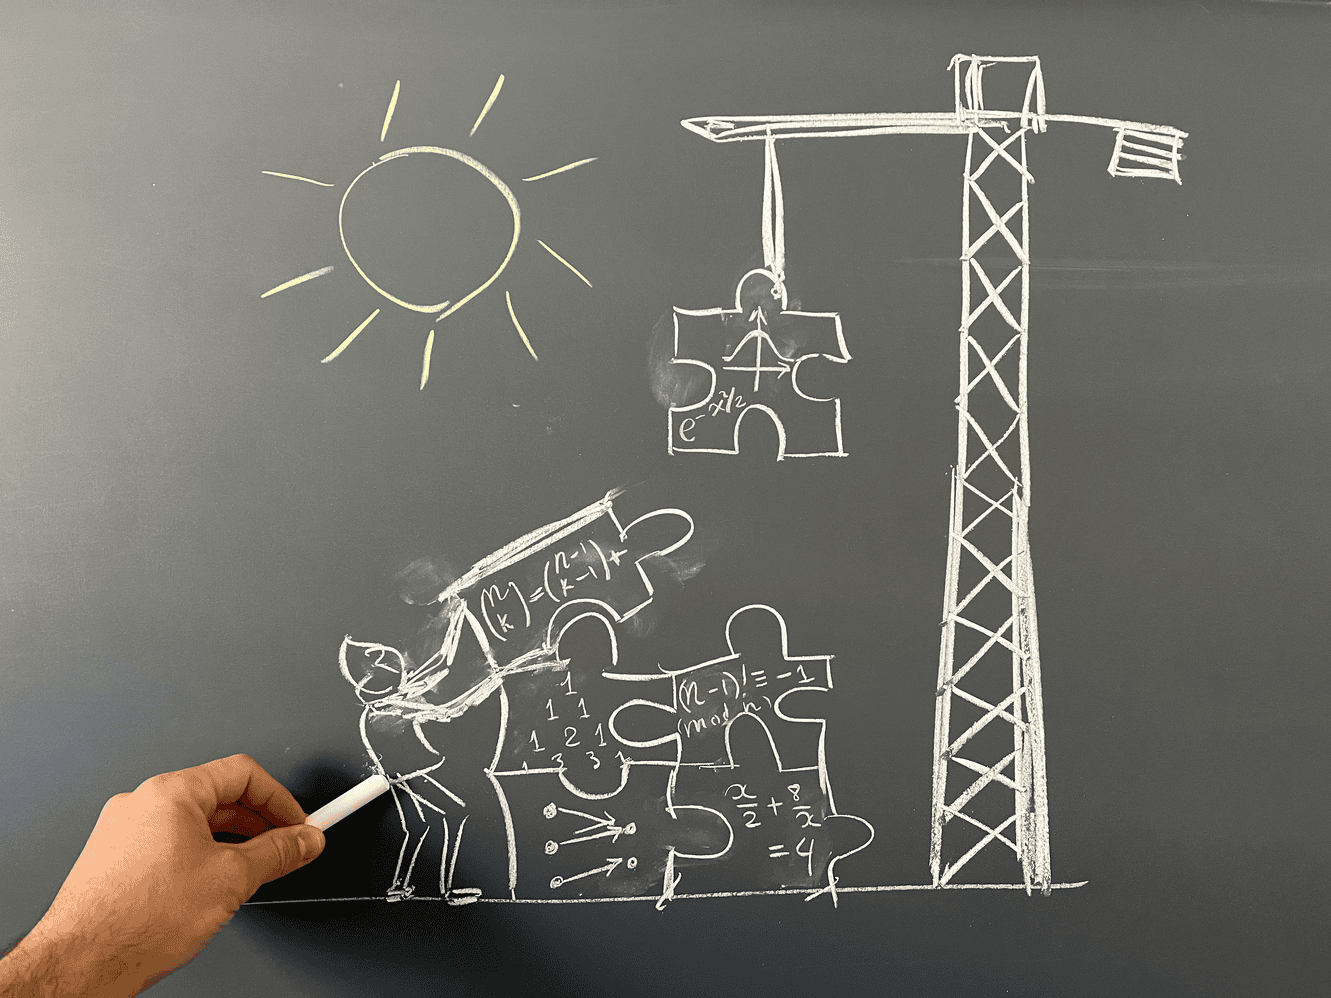
\includegraphics[width=.5\textwidth]{EGMT_image.png}
\end{center}

\newpage
\section{Contact \& Logistics}

\noindent
\begin{tabular}{ll}
\textbf{Instructor:} Leonid Petrov &\qquad \qquad \qquad\textbf{Office:} 209 Kerchof Hall \\
\textbf{Email:} \href{mailto:petrov@virginia.edu}{petrov@virginia.edu} & \qquad \qquad \qquad\textbf{Office hours:} TBA \\
\textbf{Website:} \url{https://lpetrov.cc}
\end{tabular}

\vspace{4pt}

\noindent\textbf{Meetings:} 
Mondays 3:30--6:00PM, Gilmer Hall 247
(September 1, 8, 15, 22, 29; October 6).

\medskip
\noindent
\textbf{Math debate split session:} One additional session of math debates in the weeks of September 15 and 22. 
Class split in half by poll (others welcome to attend the debate, too).

\section{How we work together}

This is a hands-on, pen-and-paper course. Each meeting begins with 
a brief review, then you receive
a fresh problem set. You work at your table in fixed small groups, develop ideas, test them, and revise when needed. I circulate, ask questions, and may invite nearby peers to listen in and challenge your reasoning.

\begin{enumerate}[$\bullet$]
  \item \textbf{Home subgroups (fixed):} On day one we form 6 ``home subgroups'' for in-class collaboration:
  $\delta, \ \theta, \ \zeta, \ \rho, \ \lambda, \ \phi$.\footnote{Math and science use Greek symbols very often. The names of the subgroups are 
	\emph{delta}, \emph{theta}, \emph{zeta}, \emph{rho}, \emph{lambda}, and \emph{phi}.}
	Groups remain stable.

  \item \textbf{In-class problem work (at the table):} At
	the start of class you receive a new problem set.
	Your group works at the table; when ready, you explain
	your solution to me. I act as a skeptical audience.
	You may use scrap paper or your commonplace book to write up your solution.
	During your subgroup's explanation, I may ask a different member to continue the explanation,
	so everyone should understand the full argument.

  \item \textbf{Random mixers:} 
		Near the end of class, we spend about 10-15 minutes 
		in randomly mixed groups.
		Quick reshuffles outside your home group allow you
		to compare partial solutions and share techniques.
		
	 \item \textbf{Mini-debate session (dedicated slot with a new
	 problem):} In a scheduled debate block (separate from
	 regular weekly work), the class receives a {new}
	 problem designed for argument-testing. There is
	 structured {work time} to develop approaches,
	 followed by {presentation and questioning}. 
	 A pair of presenters will be at the board explaining the
	 solution, while the rest of the class 
	 focuses on questioning and debating the claim.
  
	\item \textbf{Math debate:} Scheduled separately; see below for details.

	\item \textbf{Commonplace book:} Bring it every time.
	Use it for quick recaps, sketches, diagrams, partial
	proofs, and brief reflections. Photos of selected pages
	are submitted to Canvas each week (see details below).

  \item \textbf{Team roles (rotate each meeting):} In groups of $5$--$6$, 
		the following sample roles work well:
		\begin{compactitem}
			\item \textsc{Explainer}: articulates the current
			approach and restates the problem in your own words.
			\item \textsc{Skeptic}: presses on assumptions, looks
			for gaps, and frames precise questions.
			\item \textsc{Counterexample Hunter}: designs and
			tests examples/edge cases to probe the claim.
			\item \textsc{Recorder}: maintains a clean write-up in
			the commonplace book.
			\item \textsc{Verifier}: checks computations and logic, and
			ensures steps follow from the stated problem.
			\item \textsc{Connector}: ensures that all subgroup
			members understand and can explain the solution.
		\end{compactitem}
		You may keep the roles informal or explicitly assign them in your
		subgroup, but \emph{make sure you rotate them each week}.

  \item \textbf{Devices:} Please keep devices in your bag 
		unless you have an accommodation that requires otherwise.
		This is a pen-and-paper course.
\end{enumerate}

\section{Math debate}

\section{Commonplace book weekly assignments}

\begin{enumerate}[(1)]
  \item \textbf{What counted as evidence for me?}
  In $\tfrac{3}{4}$--1 page, name one claim from this week and list \emph{exactly what} made it convincing \emph{to you} (e.g., a minimal example, a failed counterexample, a definition that removed ambiguity, a lemma that closed a gap). Include one micro-diagram or worked micro-case. End with one thing that would change your mind (a potential counterexample or missing step).
  \item \textbf{Assumption audit.}
  List the assumptions you actually used (not just those stated in the problem). For each, mark: \emph{needed} / \emph{not needed} / \emph{uncertain}. Then try to \emph{drop one}: either give a tiny counterexample that shows it \emph{was} needed, or a brief note explaining why the argument still goes through. Length: about $\tfrac{1}{2}$ page.
  \item \textbf{Complete solution write-up (one problem).}
  Choose one problem \emph{designated for write-up} in the handout, and write a clear, self-contained solution (aim for 1--1.5 pages). Define terms you use, justify each step, and cite any lemmas or previously settled claims.
\end{enumerate}
\emph{Submission format:} clear photos or a single PDF to Canvas by Sunday 10:00\,pm. AI tools may be used for learning (brainstorming hints, clarifying definitions) but \emph{not} to generate text for submitted write-ups; see ``Use of AI'' policy.


\section{Grading}

\begin{enumerate}[$\bullet$]
  \item \textbf{In-class work \& explanations (35\%):}
	Attendance,
	active contribution in your subgroup, table-side explanations, 
	and participation in mini-debates and random mixers.
 
 \item \textbf{Commonplace notebook (35\%):}
	A three-part weekly writing assignment, submitted
	on Canvas by Sunday 10:00\,pm as photos or a PDF scan. 

  \item \textbf{Math debate (20\%):}
	Attendance and participation in the math debate.

	\item \textbf{Engagement experience (10\%):}
  TBD
\end{enumerate}



\section{Policies}

\subsection{Late/make up work}

Each assignment will have due date and time. Late assignments are not accepted --- there is no room for late work in our schedule. If you have special needs, emergency, or unavoidable conflicts, please let me know as soon as possible.

\subsection{Honor Code}
The University of Virginia Honor Code applies to this class and is taken seriously. Any honor code violations will be referred to the Honor Committee. 

\subsection{Devices}

This is a pen and paper course. Please keep all devices in your bag during class activities, unless you have an accommodation that requires otherwise.

\subsection{Use of AI}

USE of AI: not for class; okay for learning during homework, but not for writing up solutions.
\href{https://gist.githubusercontent.com/lenis2000/cb5ea004f8aa6461be71398e19ae488e/raw/a0103eab0b865a1cedf2f3bf3c00d217bd294005/AI_hint_prompt.txt}{\texttt{this}} is a prompt for learning: 


\subsection{Attendance}

Attendance is expected at all class meetings, including the extra meeting for math debate. If you miss a class, you are responsible for catching up on the material covered. If you have a valid reason for missing a class, please inform me in advance.

\subsection{Special needs}

All students with special needs requiring accommodations should present the appropriate paperwork from the Student Disability Access Center (SDAC). It is the student's responsibility to present this paperwork in a timely fashion and follow up with the instructor about the accommodations being offered. 

% \subsection{Recording for a personal study}
%
% Class sessions for this course may be audio recorded as a
% reasonable accommodation for a disability for the student's
% own personal study and review. These audio recordings will
% be deleted at the end of the semester. Recordings will not
% be reproduced, shared with those not enrolled in the class,
% nor uploaded to other online environments.



\end{document}
